%% grundlagen.tex
%% $Id: grundlagen.tex 61 2012-05-03 13:58:03Z bless $
%%

\chapter{Grundlagen}
\label{ch:Grundlagen}
%% ==============================
Dieses Kapitel beinhaltet grundlegende Informationen zu der Arbeit. Zuerst werden die Spielregeln erklärt, dann die verwendete Unity Engine und zum Schluss wird noch auf Formen der künstlichen Intelligenz eingegangen. Dabei wird unterschieden zwischen strategischen und deterministischen KIs, sowie dem Machine Learning.
\section{Latrunculi}
\label{ch:Grundlagen:sec:Latrunculi}
Ulrich Schaedler\cite{homoLudens} hat beschrieben, wie entzückt die Römer von diesem Spiel waren. Nicht nur zum selber spielen waren sie für Latrunculi zu begeistern, sondern wohl auch beim Zuschauen von begabten Spielern. Die heute überlieferten Regeln sind nicht ganz eindeutig geklärt, daher gibt es aktuell verschiedene Variationen dieses Spiels. Die in dieser Arbeit umgesetzte Variante orientiert sich an der von Kowalski\cite{comscigate} beschriebenen Version. Dabei gab es keine feste Größe des Spielfelds. Schädler\cite{homoLudens} berichtet von Ausgrabungen bei denen Größen wie 7x6 oder 10x10 gefunden wurden. Kowalski\cite{comscigate} erklärt die Basis-Version mit einem 8x8 Brett. Die Felder wurden in unterschiedliche Materialien geritzt. Schaedler berichtet von Kalksteinen und Marmor, aktuelle Versionen werden aber vor allem auf Holz oder Leder umgesetzt\footnote[4]{\url{https://www.spielmannshof-seitenroda.de/die-spiele/latrunculi/}}. Der Ausgangszustand wird ebenfalls unterschiedlich ausgelegt. Masters Traditional Games\cite{mastersgames} beschreibt eine Variation mit zwei Reihen an Steinen auf beiden Seiten der Spieler, wohingegen die Version von Kowalski\cite{comscigate} mit jeweils nur einer funktioniert. Weiterhin gab es Regeln bei denen zu Beginn entweder die Steine nacheinander platziert\cite{homoLudens} oder aber direkt auf den ersten Reihen gesetzt wurden. Im folgenden Abschnitt wird näher auf die umgesetzten Spielregeln eingegangen.
%% ==============================
\paragraph{Spielregeln}
%% ==============================
\label{ch:Grundlagen:sec:Spielregeln}

Der grundsätzliche Aufbau des Spiels beinhaltet ein Spielbrett mit minimum 6x6 Feldern bis hin zu 12x12 großen Brettern. Weiterhin gibt es zwei verschiedene Spielsteine, die entweder unterschiedliche Farben haben oder aus zum Beispiel einerseits Steinen und andererseits Muscheln, wie in dieser Ausarbeitung auch, bestehen. Dabei übernimmt ein Spieler die Steine und der Gegenspieler die Muscheln. Zu Beginn werden die eigenen Steine jeweils auf der ersten Reihe platziert, wie in Abbildung \ref{fig:startzustand} zu sehen ist. Das Spiel beginnt mit einem der beiden Spieler. Während des Spiels ziehen die Spieler abwechselnd horizontal oder vertikal über das Feld, ohne dabei einen anderen Stein zu überspringen oder auf einer besetzten Zelle zu landen (Abbildungen \ref{fig:Bewegungen}). Um gegnerische Spielsteine zu erobern, müssen diese wie in der Abbildung \ref{fig:erobern} von eigenen Steinen auf zwei gegenüberliegenden Feldern umstellt sein. Wird ein gegnerischer Stein erobert, dann wird dieser aus dem Spiel entfernt und ein eigener darf nochmal bewegt werden. Hierbei gibt es auch Variationen bei denen nur der zuletzt bewegte Stein sich wieder bewegen darf.
Bewegt sich ein eigener Stein zwischen zwei gegnerische und scheint somit umstellt zu sein, zählt dieser allerdings nicht als erobert(Abbildung \ref{fig:erobern}).
Das Ziel des Spiels ist es, dass der Gegenspieler keinen Zug mehr ausführen kann beziehungsweise keinen Spielstein mehr erobern kann.
\begin{figure}[h]
\centering
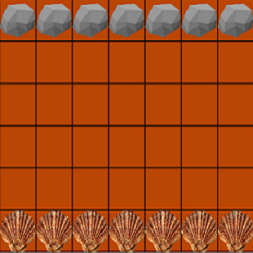
\includegraphics{img/regeln_startzustand22}
\caption{Startkonfiguration eines 7x6 Latrunculi Feldes}
\label{fig:startzustand}
\end{figure}
\begin{figure}[h]
	\centering
	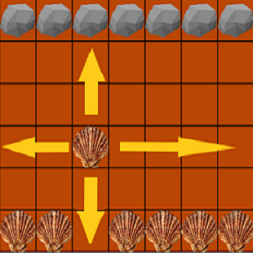
\includegraphics{img/regeln_bewegung222}
	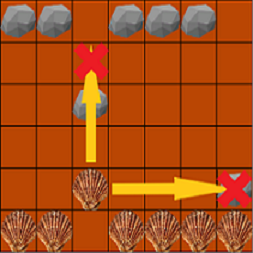
\includegraphics{img/regeln_nottodo22}
	\caption{Legitime Bewegungen auf einem 7x6 Latrunculi-Feld(links) \& nicht erlaubte Züge (rechts)}
	\label{fig:Bewegungen}
\end{figure}
\begin{figure}[h]
	\centering
	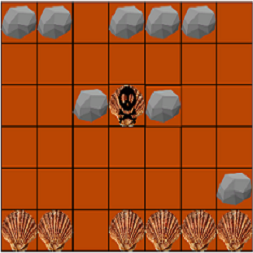
\includegraphics{img/regeln_erobern22}
	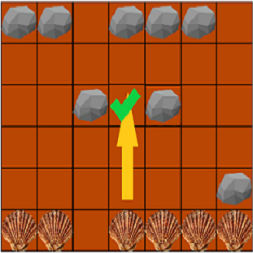
\includegraphics{img/regeln_nichterobert22}
	\caption{Eroberung eines Spielsteins(links) und keine Eroberung(rechts)}
	\label{fig:erobern}
\end{figure}
%% ==============================
%\section{Künstliche Intelligenz}
%% ==============================
%\label{ch:Grundlagen:sec:Abschnitt2}
%\nocite{computerweekly}
%\nocite{barr2014handbook}

%Der amerikanische Informatiker John McCarthy prägte 1956 den Begriff künstliche Intelligenz (KI) auf der Dartmouth Conference.
%Künstliche Intelligenz findet heutzutage in vielen Bereichen Anwendung und ist eine immer wichtigere Entwicklung, um menschliche Arbeit zu vereinfachen und auch auf Computer zu übertragen. Seit der Begriff geprägt wurde, haben sich die dazugehörigen Bereiche erweitert. Heute definiert KI die Automatisierung von Prozessen bis hin zur Robotik.
%Hierbei geht es vor allem um den Zusammenhang zwischen Berechnung und Wahrnehmung.
%Aufgrund der riesigen Datenmengen (Big Data), die ein Mensch alleine nicht bearbeiten oder analysieren kann, wird dieser Bereich immer wichtiger. Maschinen können viel effizienter Daten analysieren und Muster erkennen, als ein Mensch es könnte.\\
%Um die unterschiedlichen Typen zu kategorisieren, kann man sich die vier verschiedenen Typen, die von Arend Hintze, Assistenzprofessor für Integrative Biologie und Informatik der Michigan State University klassifiziert wurden, betrachten:

%\paragraph{Typ 1: Reaktive Maschinen}
%Zu den Reaktiven Maschinen zählen solche, die den aktuellen Zustand kennen und zukünftige Entscheidungen analysieren und bewerten können. Als Beispiel kann man sich hier Deep Blue anschauen. Deep Blue ist ein von IBM entwickeltes Schachprogramm und ist in der Lage die Figuren auf dem Spielbrett zu erkennen  und mögliche Züge beider Spieler analysieren. Da Deep Blue keine lernende Komponente enthält, werden vergangenen Spielsituationen nicht betrachtet und haben keinen Einfluss auf zukünftige Züge.

%\paragraph{Typ 2: Begrenzter Speicher}
%Zum zweiten Typen zählt man Systeme, die vergangene Erfahrungen nutzen können, allerdings werden hier Beobachtungen aus naher Zukunft nicht gespeichert. Als Beispiel können hier autonome Fahrzeuge betrachtet werden, die den Wechsel der Fahrspur eines Autos nicht dauerhaft speichern.\\
%\newline
%Die nachfolgenden beiden Typen existieren in der beschriebenen Form noch nicht:
%\paragraph{Typ 3: Native Theorie}
%Die Native Theorie ist ein psychologischer Begriff und bezeichnet Systeme, die verstehen, dass andere eigene Überzeugungen, Wünsche und Absichten haben, die ihre Entscheidungen beeinflussen.
%\paragraph{Typ 4: Selbsterkenntnis}
%Diese Kategorie umfasst Maschinen die ein Bewusstsein haben.Die sollen in der Lage sein ihren aktuellen Zustand zu verstehen und daraus Erkenntnisse über das Gefühl anderer zu ziehen.\\
%\newline
%In dieser Ausarbeitung wurde im Zusammenhang mit dem Spiel Latrunculi eine künstliche Intelligenz des Typ 1 entwickelt, die ihren aktuellen Zustand kennt und daraus Berechnungen für zukünftige Züge treffen kann.
%% ==============================
%\subsection{Künstliche Intelligenz in Videospielen}
%% ==============================
%\label{ch:Grundlagen:sec:Abschnitt3}
%\nocite{tecchannel}
%In Videospielen werden in der Regel Reaktive Maschinen verwendet. Hierbei werden mögliche Bewegungen entweder vorher definiert und abgearbeitet oder aber die Aktionen werden mit einem Punktesystem bewertet und abhängig von der Punktzahl ausgeführt. Dabei lässt sich festhalten, dass je mehr Bewertungskriterien die Aktionen bekommen, desto intelligenter wirkt die Künstliche Intelligenz. Betrachtet man die Entwicklung der Videospiele der letzten Jahre im Allgemeinen, fällt auf, dass vor Allem die Grafik weite Sprünge gemacht hat, im Vergleich dazu aber die eingesetzte KI sich nicht wesentlich verändert hat.\\
%Als Beispiel kann man sich das Strategiespiel Command \& Conquer aus dem Jahre 1996 anschauen, sowie den Nachfolger Command \& Conquer (2007) erkennt man das Problem das sich hier abzeichnet. Während sich die Grafik innerhalb der 11 Jahre wesentlich verbessert hat, verhält sich die KI noch immer ähnlich und es passieren die selben Fehler wie schon beim ersten Teil. Spieler müssen in diesem Spiel ein Hauptquartier aufbauen und von diesem aus die gegnerischen Spieler ausschalten, dabei müssen Rohstoffe gesammelt werden um die Basis weiter auszubauen. Zur Rohstoffgewinnung verfügt man über so genannte Ernter, welche automatisch den Rohstoff Tiberium suchen. Bei der Suche fahren diese teilweise ins gegnerische Hauptquartier und werden dort zerstört. Im Nachfolger, elf Jahre später, verhalten sich die Ernter noch immer ähnlich und die Fehler passieren hier ebenfalls, allerdings mit dem Unterschied, dass das Spiel, der Ernter und die Explosions-Animation grafisch realistischer aussehen. Wenn man hier eine lernende Komponente implementieren würde, dann könnten solche Probleme der KI zwar noch passieren, aber auf Dauer wäre Sie in der Lage, das als Fehler zu erkennen. \\

%\paragraph{MiniMax-Algorithmus}
%Der Minimax-Algorithmus dient der Entscheidungsfindung eines optimalen Spielzuges vor allem in Zwei-Spieler Spielen wie Schach oder Backgammon bei denen sich die Spieler mit ihren Zügen abwechseln. Effizient angewendet werden kann der Algorithmus vor Allem in \textbf{Nullsummenspielen}.\\
%Ein Spiel ist ein \textbf{Nullsummenspiel}, wenn die Summe aus Gewinnn und Verlust aller Spieler nach Spielende Null ergibt, das heißt der Gewinn eines Spielers ist der Verlust beziehungsweise die Niederlage eines anderen.\cite{AlphaBeta}.\\
%Diesen Algorithmus kann man sich als Spielbaum vorstellen, der mit jedem Pfad einen denkbaren Spielverlauf darstellt. Dabei repräsentiert jeder Knoten des Baumes einen Spielzustand und enthält Informationen über die Verteilung der Figuren auf dem Spielbrett, welcher Spieler am Zug ist und über mögliche weitere Spielzüge. Jeder dieser Züge ist ebenfalls wieder ein Knoten und Kind der vorherigen Aktion.

%\subparagraph{Beispiel 2.1:}
%Am einfachsten kann man sich die Funktionsweise am Beispiel von TicTacToe klar machen:\\
%Dabei repräsentiert wieder jeder Knoten, der hier als Abbildung des Spielbretts dargestellt wird, einen Zustand des Spiels. Die Bewertung der Zustände ist in diesem Spiel vergleichsweise simpel:\\
%\begin{itemize}
%	\item Spieler 1 gewinnt: +1 Punkt,
%	\item Unentschieden: 0 Punkte,
%	\item Spieler 2 gewinnt: -1 Punkt
%\end{itemize}
%\begin{figure}[h]
%	\centering
%	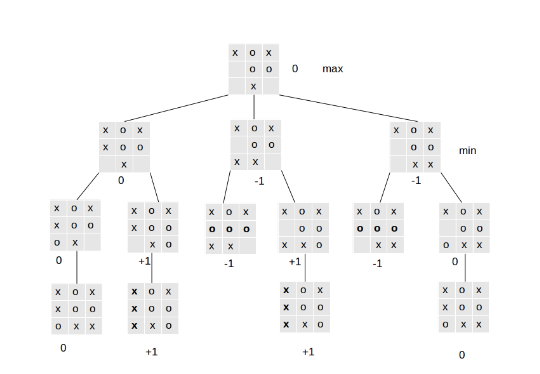
\includegraphics{img/Baum}
%	\caption{TicTacToe Spielbaum}
%	\cite{AlphaBeta}
%	\label{fig:Suchbaum}
%\end{figure}
%Der Algorithmus basiert auf der Idee, anhand dieses Baumes den Verlauf mit dem höchsten Wert zu verfolgen und so das Spiel zu gewinnnen. Dabei wird wie in Abbildung \ref{fig:Suchbaum} zu sehen, jedem Knoten ein Wert zugeordnet und versucht immer den höchstmöglichen Wert zu erzielen, wenn der Spieler gewinnen soll.

%\paragraph{Analyse \& Variationen}
%Aufgrund von tendenziell hoher Laufzeit, vor Allem bei komplexeren Spielen, gibt es verschiedene Variationen dieses Algorithmus.
%In der Basis-Version des MiniMax enden die möglichen Verläufe im ungünstigsten Fall nach $d$ Zügen, wobei $d$ für die Suchtiefe im Baum steht. Im extremsten Fall können wir annehmen, dass aus jedem Zustand weitere $w$ Züge möglich sind. Daraus resultieren auf der untersten Ebene $ w ^d$ Knoten und es gilt \[ \sum_{i=1}^d  w^{d}\in O(w^d).\]\\
%Zur Optimierung existieren unterschiedliche Variationen von denen eine hier näher beschrieben wird.
%\paragraph{Alpha-Beta-Algorithmus}
%Aufgrund der hohen Komplexität wird auch der \textbf{Alpha-Beta-Algorithmus} verwendet. Dieser basiert auf dem MiniMax-Algorithmus, allerdings wird hier der Wert der möglichen Endzustände geschätzt und die Berechnnung eines Pfads abgebrochen, sobald klar ist, dass dieser Weg weniger zielführend ist. Dabei wird angenommen, dass Zweige ab einem Punkt in der Berechnung vernachlässigt werden können. Am nachfolgenden Beispiel wird die Idee deutlicher:
%\subparagraph{Beispiel 2.2:}
%Nach der Durchsuchung des linken Teilbaums, sieht man, dass der der Ausgangsknoten mindestens den Wert 3 hat. Deshalb wird die Evaluation des rechten Teilbaums abgebrochen, sobald klar wird, dass der min-Knoten maximal einen Wert von 2 hat. Die Suche kann abgebrochen werde, da der rechte Teilbaum keine Auswirkungen auf den Startknoten hat\nocite{AlphaBeta}.
%\begin{figure}[h]
%	\centering
%	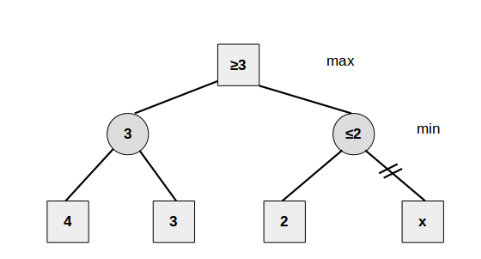
\includegraphics{img/AlphaBeta}
%	\caption{Alpha-Beta Spielbaum}
%	\cite{AlphaBeta}
%	\label{fig:AlphaBeta}
%\end{figure}
%% ==============================
\section{Unity Engine}
%% ==============================
\label{ch:Grundlagen:sec:Unity}
Die Unity Engine ist eine von Unity Technologies entwickelte Laufzeit- und Entwicklungsumgebung für Videospiele. Die Engine bietet dabei Portierungen für PCs, Spielkonsolen, mobile Geräte wie Android und Webbrowser. Bekannte Spiele wie Pokemon Go und Hearthstone wurden mit Unity entwickelt. Weiterhin bietet Unity die Möglichkeit sowohl in 2D, als auch in 3D Spiele umzusetzen und bietet Funktionen, wie den Eventhandler für Gameobjects, um die Entwicklung zu vereinfachen. Um selbstgeschriebene Skripte einzubinden, unterstützt Unity unter anderem C\#, wie ich es in dieser Arbeit auch verwendet habe. Unity wurde hier vor allem wegen der einfachen Portierung und Wiederverwendbarkeit von vorher erstellten Prefabs genutzt. Ausserdem bietet Unity eine große Anzahl an Libraries zur Unterstützung der Spielentwicklung. \\Die Engine bietet die Möglichkeit einerseits per Drag \& Drop Spielobjekte im Editor zu platzieren und diesen Objekten so ihren Ausgangszustand zu geben, andererseits gibt es Mittel die Szene dynamisch via Skript zu erstellen. Entwickelt man in der 2D Umgebung, hat man die Möglichkeit seinen Objekten Sprites mitzugeben. Diese Sprites sind Grafikobjekte, die zur Darstellung der Spielobjekte im Editor platziert werden. Selbst erstellte Skripte, Sprites und Szenen, sowie andere genutzte Ressourcen, wie zuvor erstellte Prefabs für eine dynamische Generierung, befinden sich bei Unity-Projekten im Assets-Verzeichniss.%In einem Unity Projekt befindet sich ein Ordner ,,Assets'' in dem alle selbst erstellten Skripte, Sprites und Szenen enthalten sind, sowie andere genutzte Ressourcen wie zuvor erstellte Prefabs für eine dynamische Generierung.

\paragraph{Prefab System}
\nocite{UPrefabs}
Unitys Prefab System ermöglicht es Spielobjekte zu erstellen und als Prefabs zu speichern. Diese können wiederverwendet werden und fungieren wie eine Vorlage(Template) eines Objektes. Dadurch können wiederkehrende Spielobjekte einmalig definiert werden und durch das Prefab in der selben Form oder aber auch verändert mehrfach genutzt werden. Das heißt es können dadurch zur Laufzeit Spielobjekte instanziiert und zur Szene hinzugefügt werden, ohne jedes einzelne Objekt neu zu definieren. Weiterhin können diese so erstellten Objekte trotzdem noch separat verändert werden. \nocite{UPrefabs}

%% ==============================
\section{Künstliche Intelligenz}
%% ==============================#
\label{ch:Grundlagen:sec:Künstliche Intelligenz}
Allgemein kann man sagen, dass es drei Formen der künstlichen Intelligenz gibt. Zum einen sollte man zwischen deterministischen und strategischen KIs unterscheiden, andererseits kann man diese vom Machine Learning abgrenzen.

\subsection{Strategische KIs}
\label{ch:Grundlagen:sec:strategisch}
\textbf{Strategische KIs} werden in Videospielen zum Beispiel zur Wegfindung oder für die Atmosphäre genutzt. Am Beispiel von sogenannten Non-Player-Character (kurz:NPC) in Rollenspielen wie Gothic kann diese Form  gut erklärt werden. NPCs sind Figuren innerhalb eines Spiels mit denen in der Regel interagiert werden kann oder die für die Atmosphäre eingesetzt werden und nur einen Weg ablaufen, der via Wegfinde-Algorithmus berechnet wird. Außerdem kann auch das Verhalten beeinflusst werden, indem die Spielfiguren auf Aktionen reagieren können und in einen entsprechenden Zustand versetzt werden. Betrachtet man das Spiel Gothic, erkennt man sehr leicht dieses Prinzip. Hier ist es möglich, dass der Spieler durch sein Verhalten die NPCs beeinflusst. Es existieren Figuren, die einem aggressiv gegenübertreten, falls man zum Beispiel zuvor aus seinem Haus etwas gestohlen hat. Für diese NPCs werden strategische KIs eingesetzt, um vor allem die Handlung zu unterstützen.

\subsection{Deterministische KIs}
\label{ch:Grundlagen:sec:deterministisch}
\textbf{Deterministische KIs} können Anwendung in Brettspielen finden. Hier werden Algorithmen verwendet um den Spielzustand und zukünftige zu bewerten und daraus die optimale Aktion zu finden. Diese Systeme können als Baumstruktur dargestellt werden. Die Algorithmen wurden schon erfolgreich in Spielen wie Tic-Tac-Toe oder Schach\cite{yannakakis2018artificial} verwendet. Damit diese gut funktionieren ist die Voraussetzung, dass perfekte Informationen über das Spiel vorliegen. Ein Spiel mit perfekter Information ist zum Beispiel das Spiel GO oder Schach. Hier haben die Spieler immer die Informationen über den Spielzustand und den vorherigen Zügen. Als Gegenbeispiel kann man an dieser Stelle Poker nennen, wo die Spieler immer nur ihre eigenen Karten auf der Hand kennen. Da Latrunculi ein Spiel mit perfekter Information ist wurde in dieser Arbeit der MiniMax-Algorithmus implementiert.

\paragraph{MiniMax}
Beim MiniMax-Algorithmus entspricht der Ausgangsknoten dem aktuellen Zustand und jedes Kind steht für einen zukünftigen. Diese Zustände werden nach verschiedenen Kriterien bewertet und so eine Punktzahl für jeden errechnet. An der Abbildung \ref{fig:Spielbaum} wird das Prinzip deutlicher. Dabei ist im Ausgangszustand Spieler 1 an der Reihe gewesen. Die drei abgebildeten Kinder sind jeweils mögliche Züge des zweiten Spielers. Der linke Zustand hat die Wertung 0, da hier weder eine Bedrohung oder ein Abzug aus einer Bedrohung, noch ein Angriff stattfindet. Die beiden anderen Kinder haben eine Wertung von +30, da diese Zustände zu einer Bedrohung der Muscheln führen. Die nächste Reihe zeigt mögliche Züge der Steine, die aus den vorherigen Situationen resultieren. Dabei werden Züge mit 40 bewertet, falls eine Muschel sich neben die bedrohte stellt und diese dadurch vor einer Eroberung schützt. Die höchste Bewertung 100 erhalten die Züge, die den gegnerischen Stein erobern. Diese Bewertungen werden von den höchsten Punktzahlen ausgehend bis zum Ausgangsknoten aufsummiert und ergeben dabei eine Höchstpunktzahl von -40 bei einer Suchtiefe von 2. %In diesem Fall gibt es zwei mögliche Pfade mit der höchsten Wertung. %Also muss für eine Entscheidung noch ein Zufallsgenerator eingesetzt werden der zwischen den beiden möglichen Zügen entscheidet.
\begin{figure}[h]
	\centering
	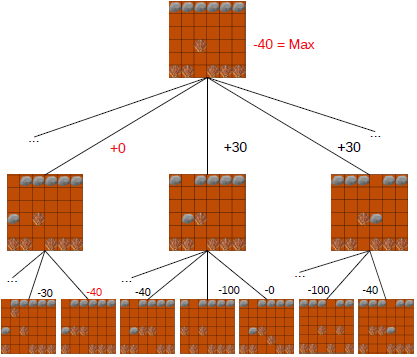
\includegraphics{img/Spielbaum_latrun4}
	\caption{ Ausschnitt: MinMax-Spielbaum eines 6x6 Latrunculi Feldes}
	\label{fig:Spielbaum}
\end{figure}
\paragraph{Erfolgreiche Umsetzungen}
Yannakakis und Togelius erwähnen in ihrem Buch ,,Artificial intelligence and games'', das der MiniMax Algorithmus an Effizienz verliert, je komplexer das Spiel ist. Die Schwierigkeit liegt darin, eine gute Evaluierungsfunktion der Zustände zu finden\cite{yannakakis2018artificial}. Je mehr Züge existieren, desto schwerer wird es eine sinnvolle Punkteverteilung zu finden. Vergleicht man Schach und Go wird das Problem deutlich. Bei ersterem hat man in der Regel über 30 mögliche Züge, diese sind im Vergleich zu Go mit bis zu 300 Möglichkeiten viel geringer. Für diese weniger komplexen Spiele gibt es bereits seit Jahren erfolgreiche Umsetzungen. IBM's entwickelte KI Deep Blue (vgl. \cite{DBLP:journals/micro/Hsu99}) hat im Mai 1997 als erster Computer den damals amtierenden Weltmeister im Schach geschlagen\cite{DBLP:journals/cse/Hsu06}. Allerdings war dies mit einem hohen Rechenaufwand und speziellen Schach-Chips verbunden(vgl. \cite{DBLP:journals/micro/Hsu99} \& \cite{DBLP:journals/cse/Hsu06}).
Festhalten lässt sich, dass der Erfolg des Algorithmus von der Evaluierungs-Funktion und von der Rechenkraft des Computers abhängig ist.

\subsection{Abgrenzung zum Machine Learning}
\label{ch:Grundlagen:sec:Learning}
Beim Machine Learning wird eine statistische Wissenbasis aufgebaut, indem das System mit Daten trainiert wird. Es ist ein Verfahren, dass Algorithmen nutzt um Daten zu analysieren und zu kategorisieren. Als Beispiel kann die Gesichtserkennung genannt werden. Hier werden die Systeme mit unterschiedlichen Gesichtern trainiert, um anschließend diese erkennen und zuordnen zu können. Generell kann man festhalten, dass diese Verfahren eher nicht in Videospielen angewendet werden. Es lässt sich zwischen dem Supervised Learning (überwachtes Lernen) und dem Unsupervised Learning (nicht überwachtes Lernen) unterscheiden.
%\paragraph{Supervised Learning}
Das überwachte funktioniert so, dass ein Algorithmus Trainingsdaten erhält, sowie die Bedeutung der Daten. Dadurch soll der Algorithmus Muster erkennen und in einer Funktion speichern, um anschließend diese Muster auf neuen Daten erkennen zu können. Diese Funktion wird abhängig von der Trefferquote vom System angepasst.
%\paragraph{Unsupervised Learning}
Beim nicht überwachten Lernen werden nicht kategorisierte Daten dem Algorithmus übergeben, sodass dieser Cluster erkennen soll und zukünftige Daten einordnen kann.\\

%\paragraph{Reinforcement Learning}


%Die künstliche Intelligenz in digitalen Brettspielen funktioniert mit einem Bewertungssystem, dabei kalkuliert man die möglichen Züge. Dieses Ranking wird dann mit entsprechenden Algorithmen wie dem MinMax evaluiert. Diese kann man sich wie einen Baum vorstellen (Abbildung \textbf{TODO}). Dabei entspricht jeder Knoten einem Spielzustand und berechnet je nach festgelegter Tiefe mögliche Verläufe. Für die Bewertung müssen sinnvolle Kriterien festgelegt werden um entscheiden zu können ob der betrachtete Zug einen Spielvorteil bringt. 


%% ==============================
%%\section{State of the Art}
%% ==============================
%\label{ch:Grundlagen:sec:SOTA}
%Die Literaturrecherche soll so vollständig wie möglich sein und bereits existierende relevante Ansätze (Verwandte Arbeiten / State of the Art / Stand der Technik) beschreiben bzw. kurz vorstellen.
%Es soll aufgezeigt werden, wo diese Ansätze Defizite aufweisen oder nicht anwendbar sind, z.B. weil sie von anderen Umgebungen oder Voraussetzungen ausgehen.

%Je nach Art der Abschlussarbeit kann es auch sinnvoll sein, diesen Abschnitt in die Einleitung zu integrieren oder als eigenes Kapitel aufzuführen.

%%Beispiel, wie mit LaTeX zitiert werden kann: \cite{TB98,JSAC96,qosr} \cite{AlphaBeta}

%%% Local Variables: 
%%% mode: latex
%%% TeX-master: "thesis"
%%% End: 
